The results from the search for non-resonant Higgs bosons pair
production presented in~\Cref{sec:dihiggs} was reinterpreted by the
ATLAS collaboration in the context of possible variations of the Higgs
boson self-coupling constant \lambdahhh in
Ref.~\cite{ATLAS-CONF-2021-052}.

anomalous couplings

Self-coupling modifier~$\klambda = \lambdahhh / \lambdahhh^{\text{SM}}$.

\todo[inline]{Read YR about Higgs cross section predictions:
  \url{https://cds.cern.ch/record/2227475/files/CERN-2017-002-M.pdf}}


\begin{figure}[htbp]
  \begin{subfigure}{0.495\textwidth}
    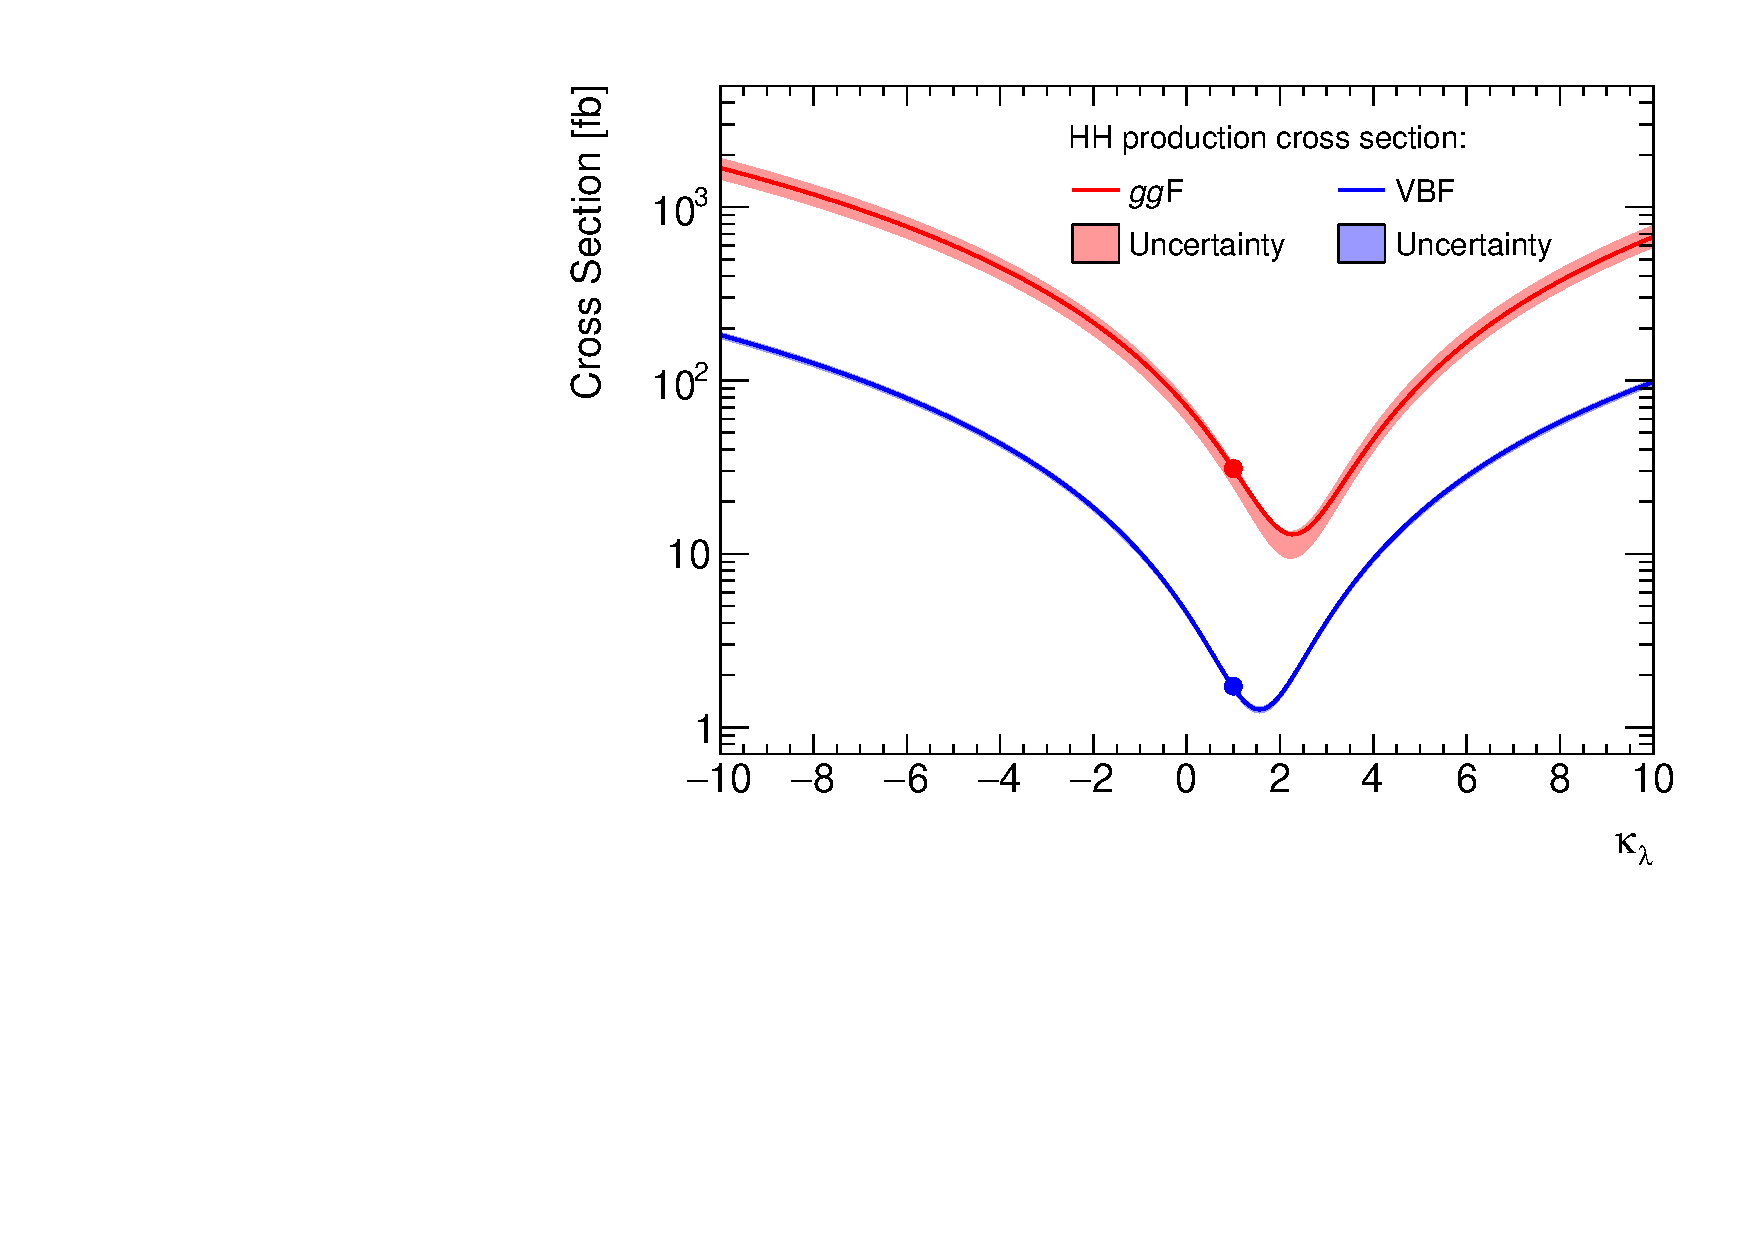
\includegraphics[width=\textwidth]{self_coupling/hh_xsec}
    \subcaption{Inclusive cross section of \HH production via \ggF and
      VBF as a function of \klambda. Theory cross section
      recommendations of the ``LHC Higgs Working
      Group''~\cite{LHCHWGHH} are adopted. For \ggF, the cross section
      is given at
      $\text{NNLO}_{\text{NLO-improved}}$~\cite{Amoroso:2020lgh}
      scaled to $\text{NNLO}_{\text{FTapprox}}$ in the $\klambda = 1$
      limit.}%
    \label{fig:hh_xsec_incl}
  \end{subfigure}\hfill%
  \begin{subfigure}{0.495\textwidth}
    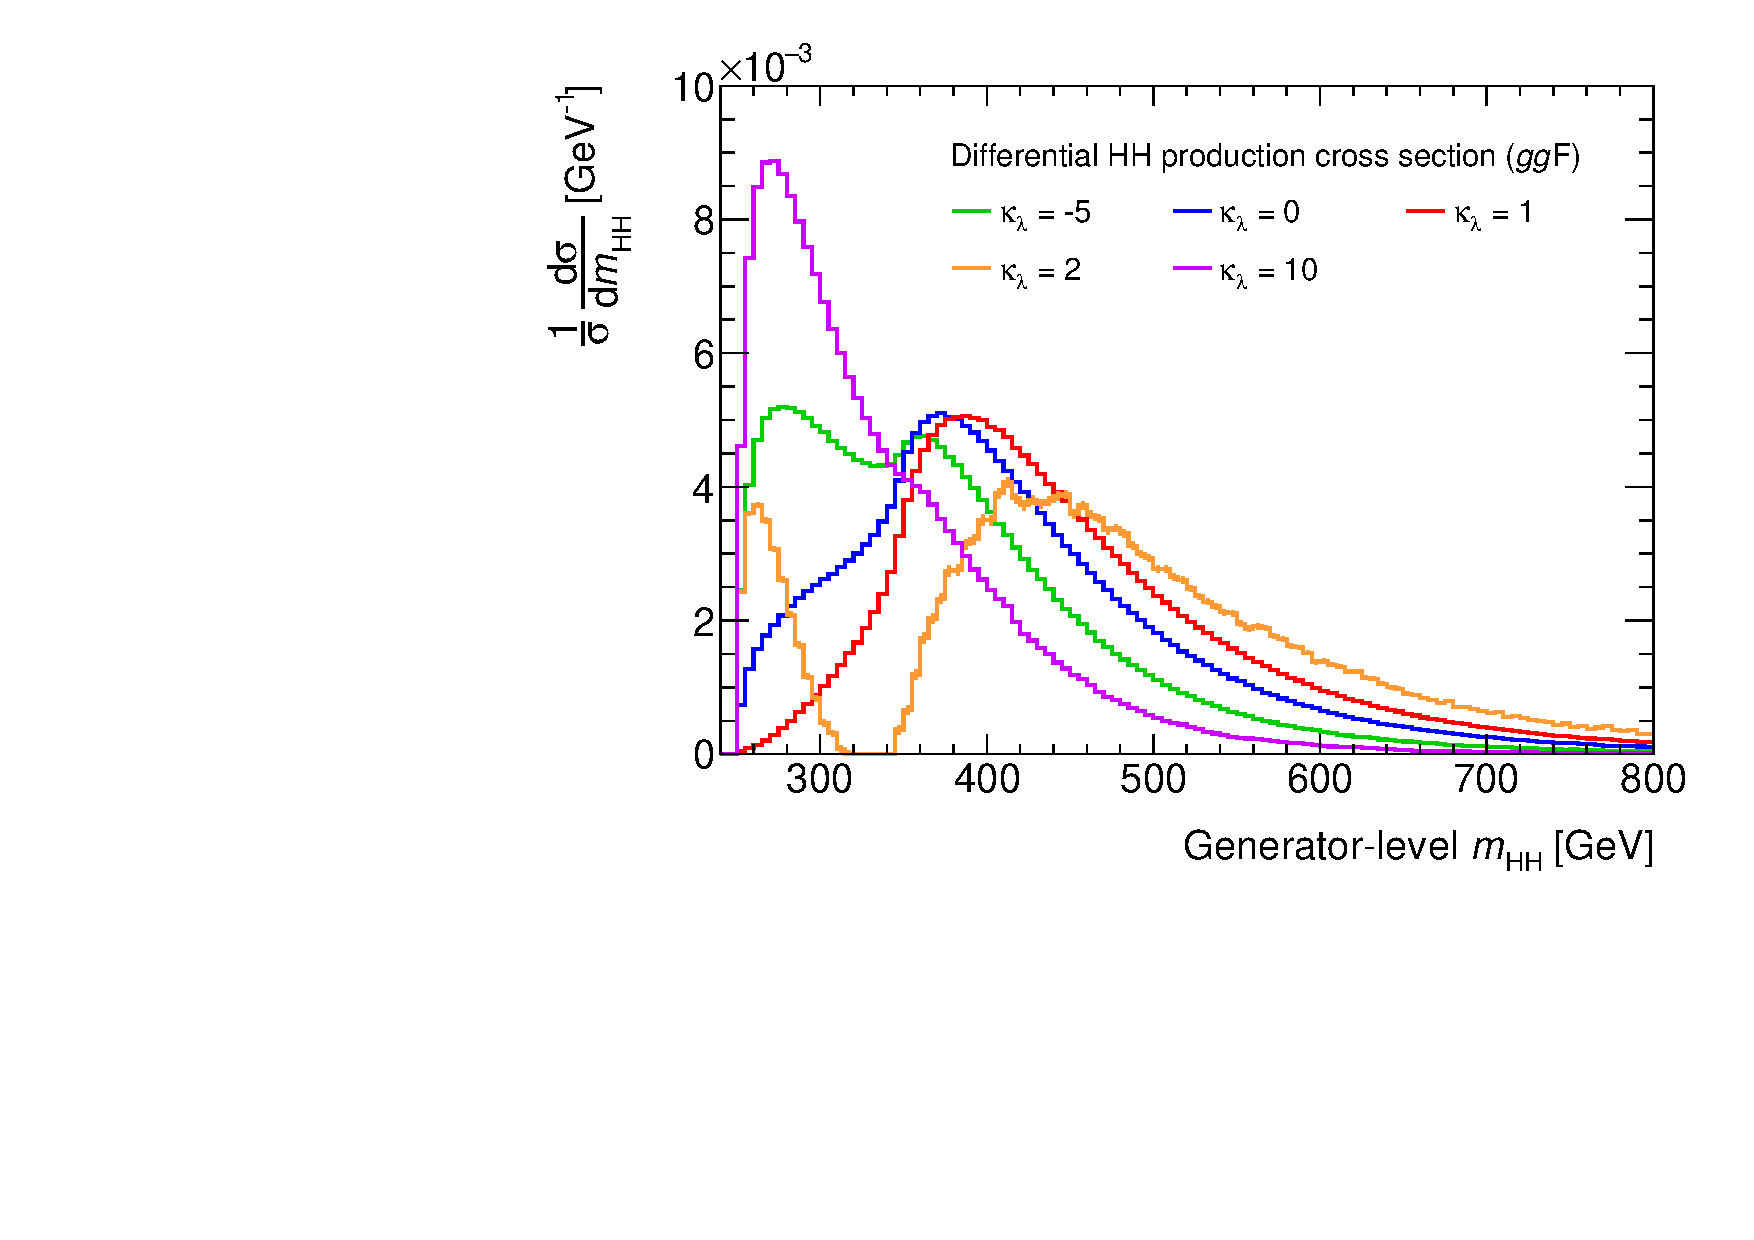
\includegraphics[width=\textwidth]{self_coupling/hh_mhh_vs_klam}
    \subcaption{}
  \end{subfigure}

  \caption{Higgs boson pair production cross sections for
    $\mH = \SI{125.0}{\GeV}$ in $pp$-collisions at
    $\sqrt{s} = \SI{13}{\TeV}$. The Higgs boson self-coupling
    modifier, \klambda.
  }%
  \label{fig:hh_xsec_vs_klam}
\end{figure}

\todo[inline]{Hadhad channel: Acceptance times efficiency vs mHH.}

\todo[inline]{Hadhad channel: Acceptance times efficiency vs kLambda.}












%%% Local Variables:
%%% mode: latex
%%% TeX-master: "../../phd_thesis"
%%% End:
